% =============================================================================
% Alternative-estimator robustness figures
% Each figure shows the event study from three estimators:
%   (a) Chaisemartin & D'Hautfeuille
%   (b) Gardner
%   (c) Wooldridge
% Callaway & Sant'Anna is excluded — it appears as the headline figure.
%
% First block (3 figures): ENUSC survey outcomes
% Second block (1 figure): SPD administrative crime outcomes
% =============================================================================


% ----- Victimization (delitos) -----------------------------------------------
\begin{figure}[h!]
    \centering
    \caption[Effects of \emph{Plan Cuadrante} on Victimization Using Alternative Estimators]{Effects of \emph{Plan Cuadrante} on Victimization Using Alternative Estimators}
    \label{fig:alterestim_delitos}
    \begin{subfigure}{0.47\textwidth}
        \centering
        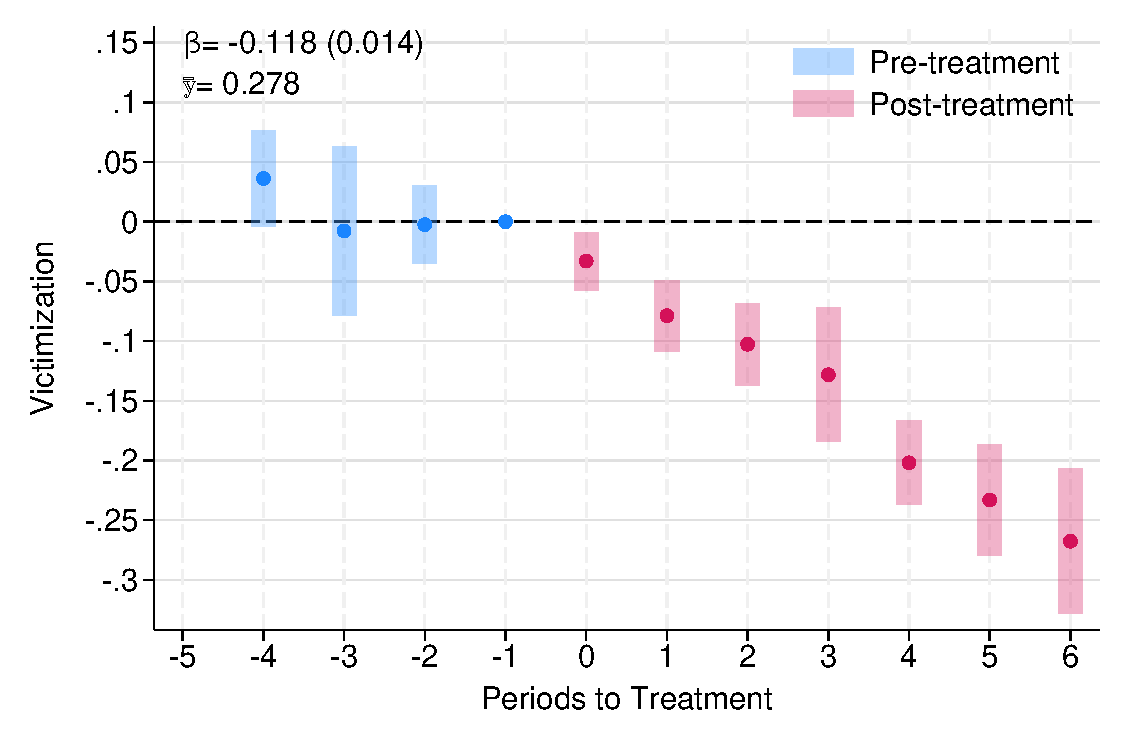
\includegraphics[width=\textwidth]{../manuscript/Graphs/CHDH_event_study_delitos.pdf}
        \caption{Chaisemartin \& D'Hautfeuille}
    \end{subfigure}%
    \begin{subfigure}{0.47\textwidth}
        \centering
        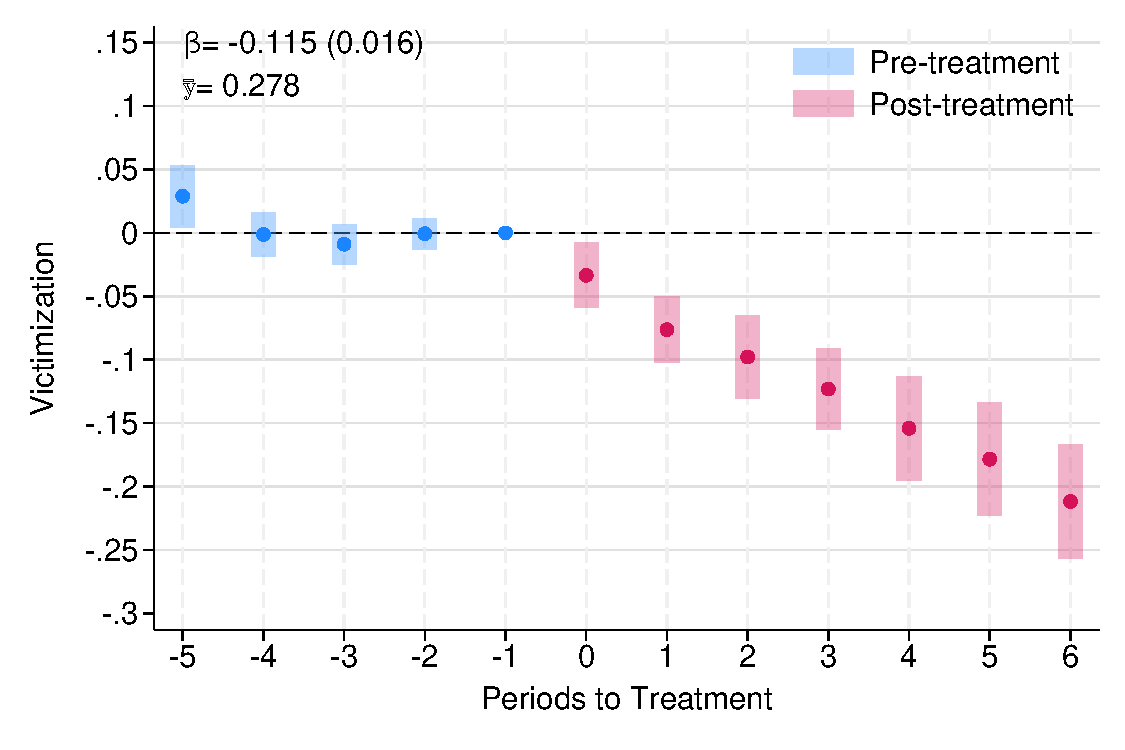
\includegraphics[width=\textwidth]{../manuscript/Graphs/DID2S_event_study_delitos.pdf}
        \caption{Gardner}
    \end{subfigure}
    \\[6pt]
    \begin{subfigure}{0.47\textwidth}
        \centering
        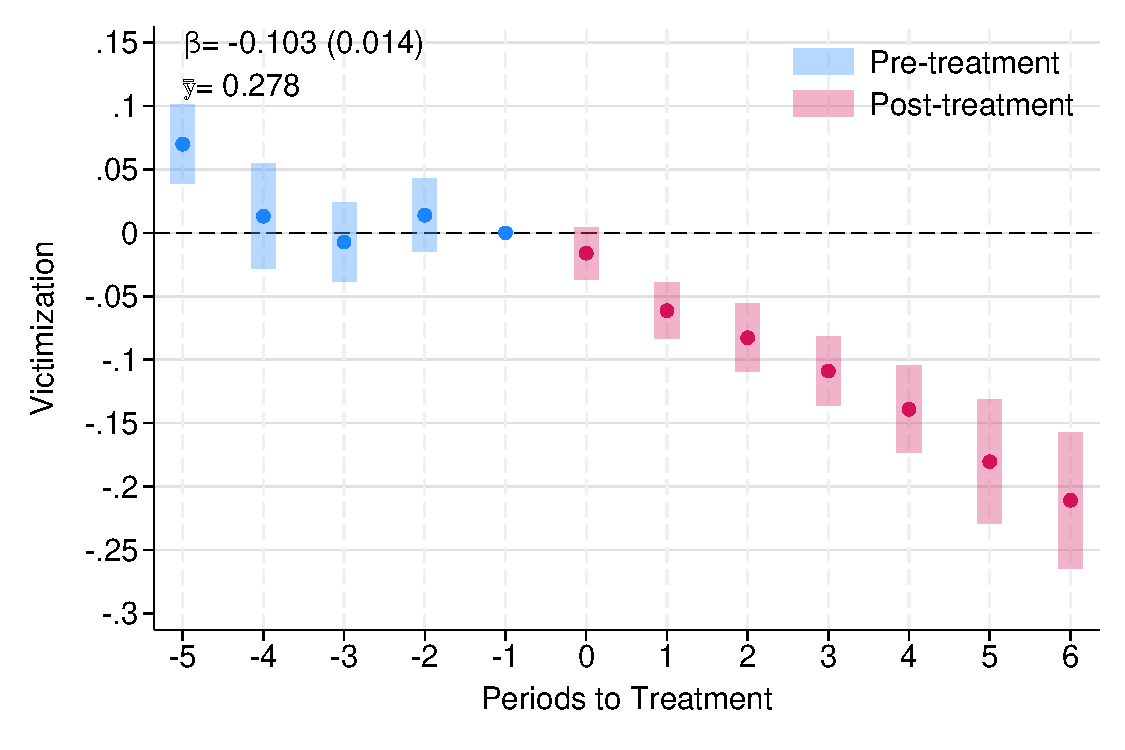
\includegraphics[width=\textwidth]{../manuscript/Graphs/JWDID_event_study_delitos.pdf}
        \caption{Wooldridge}
    \end{subfigure}
    \\[12pt]
    \begin{minipage}{0.99\textwidth}
    \footnotesize Notes: The figure reports event-study estimates of the effect of \emph{Plan Cuadrante} on the probability of household victimization in the last 12 months using the ENUSC survey, estimated with three alternative difference-in-differences estimators robust to staggered adoption: \citet{Chaisemartin} in panel (a), \citet{Gardner} in panel (b), and \citet{wooldridge2023simple} in panel (c). Each panel plots the estimated coefficient at each event time relative to treatment along with 95\% confidence intervals. Standard errors are clustered at the municipality level. The headline coefficient $\beta$ corresponds to the average post-treatment effect, and $\bar{y}$ denotes the never-treated mean of the outcome over the sample period.
    \end{minipage}
\end{figure}


% ----- Crime perception (inseguridad_barrio1) --------------------------------
\begin{figure}[h!]
    \centering
    \caption[Effects of \emph{Plan Cuadrante} on Crime Perception Using Alternative Estimators]{Effects of \emph{Plan Cuadrante} on Crime Perception Using Alternative Estimators}
    \label{fig:alterestim_inseguridad}
    \begin{subfigure}{0.47\textwidth}
        \centering
        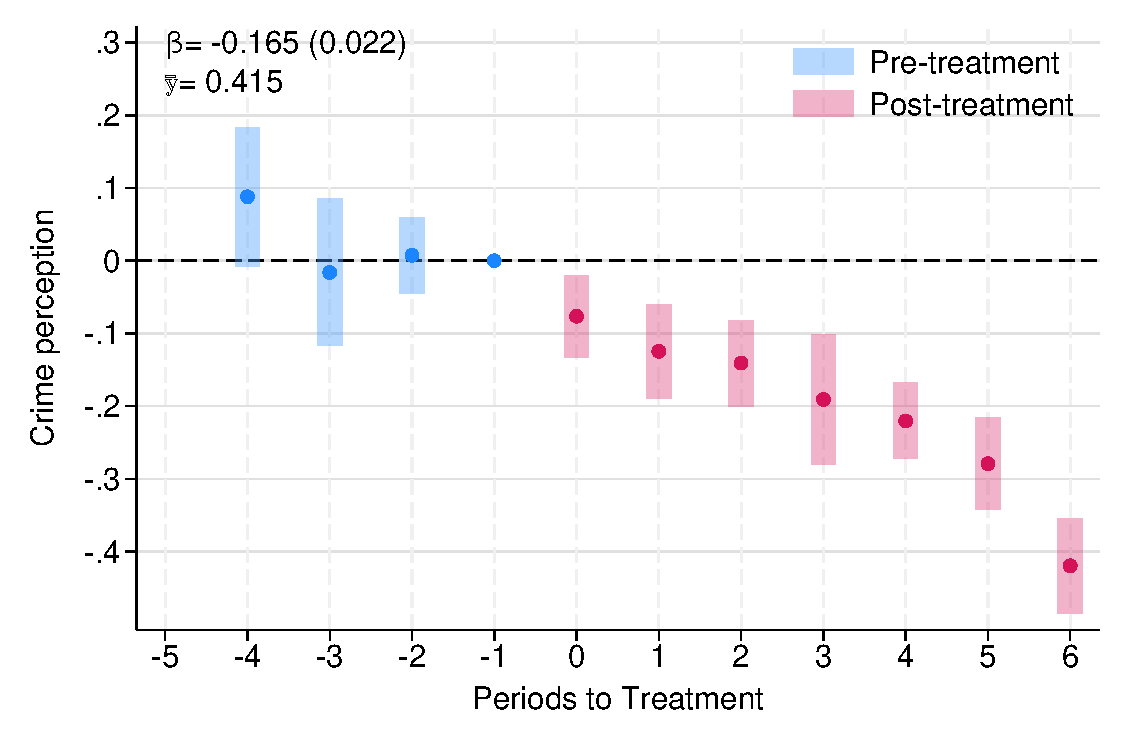
\includegraphics[width=\textwidth]{../manuscript/Graphs/CHDH_event_study_inseguridad_barrio1.pdf}
        \caption{Chaisemartin \& D'Hautfeuille}
    \end{subfigure}%
    \begin{subfigure}{0.47\textwidth}
        \centering
        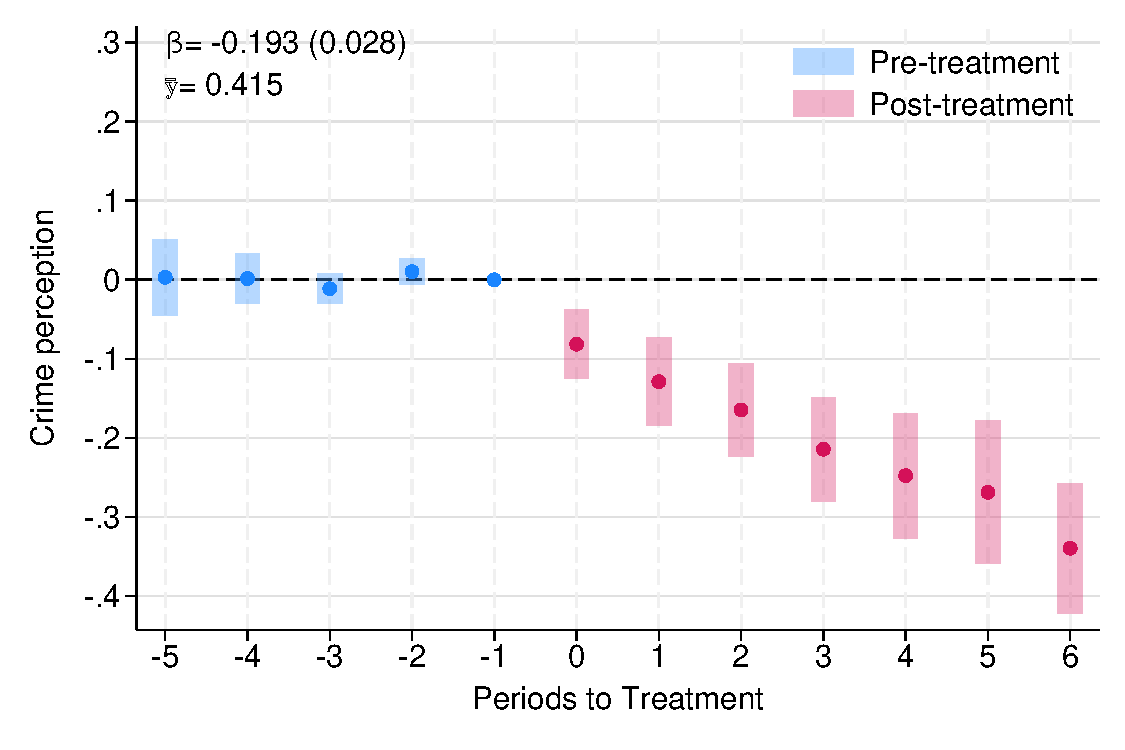
\includegraphics[width=\textwidth]{../manuscript/Graphs/DID2S_event_study_inseguridad_barrio1.pdf}
        \caption{Gardner}
    \end{subfigure}
    \\[6pt]
    \begin{subfigure}{0.47\textwidth}
        \centering
        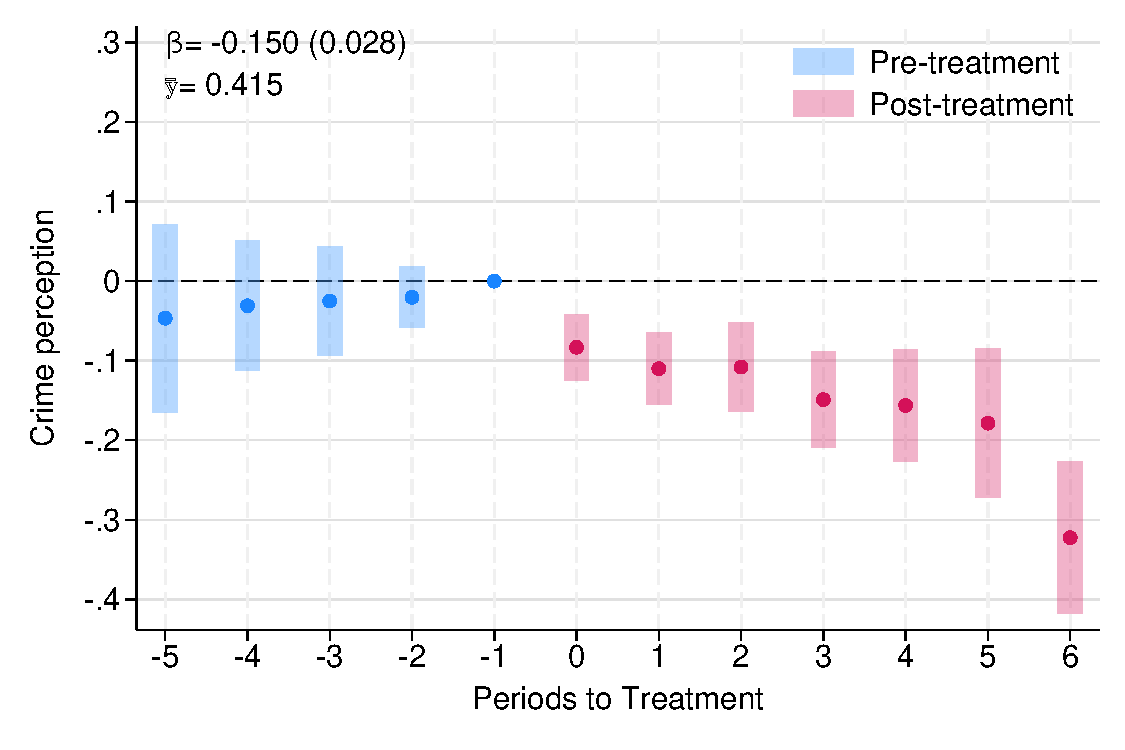
\includegraphics[width=\textwidth]{../manuscript/Graphs/JWDID_event_study_inseguridad_barrio1.pdf}
        \caption{Wooldridge}
    \end{subfigure}
    \\[12pt]
    \begin{minipage}{0.99\textwidth}
    \footnotesize Notes: The figure reports event-study estimates of the effect of \emph{Plan Cuadrante} on the probability of perceiving an increase in crime using the ENUSC survey, estimated with three alternative difference-in-differences estimators robust to staggered adoption: \citet{Chaisemartin} in panel (a), \citet{Gardner} in panel (b), and \citet{wooldridge2023simple} in panel (c). Each panel plots the estimated coefficient at each event time relative to treatment along with 95\% confidence intervals. Standard errors are clustered at the municipality level. The headline coefficient $\beta$ corresponds to the average post-treatment effect, and $\bar{y}$ denotes the never-treated mean of the outcome over the sample period.
    \end{minipage}
\end{figure}


% ----- Private investment in security (medidas_general_12) -------------------
\begin{figure}[h!]
    \centering
    \caption[Effects of \emph{Plan Cuadrante} on Investment in Security Measures Using Alternative Estimators]{Effects of \emph{Plan Cuadrante} on Investment in Security Measures Using Alternative Estimators}
    \label{fig:alterestim_medidas}
    \begin{subfigure}{0.47\textwidth}
        \centering
        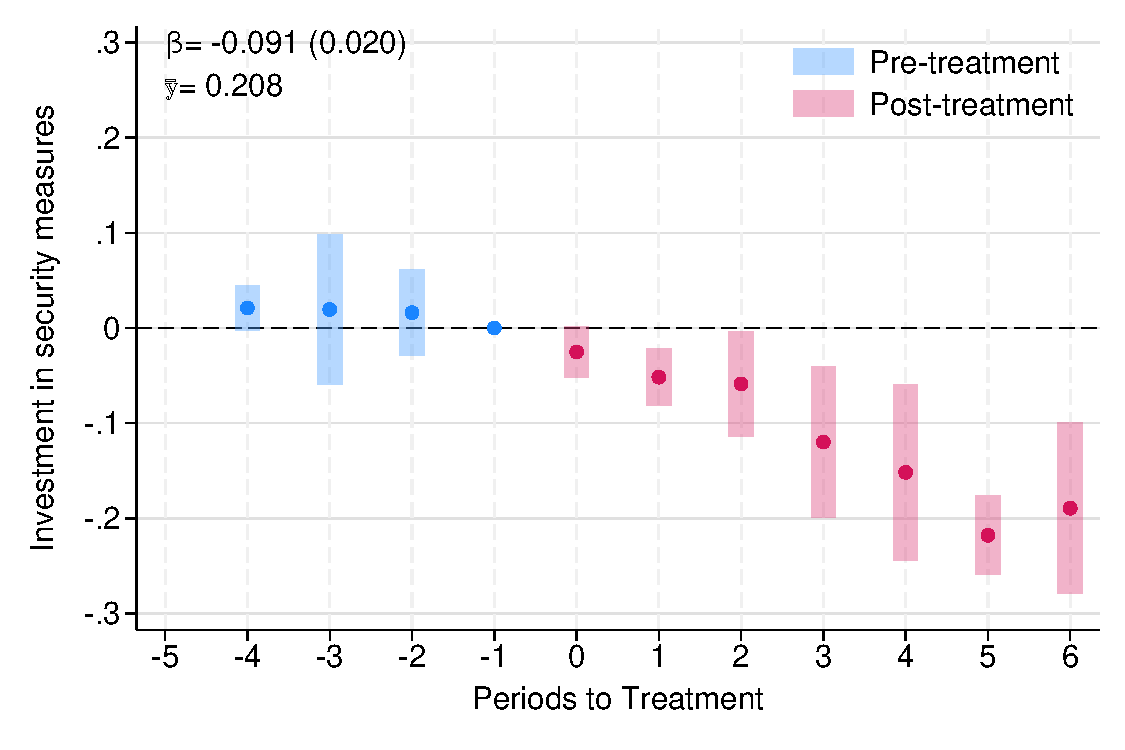
\includegraphics[width=\textwidth]{../manuscript/Graphs/CHDH_event_study_medidas_general_12.pdf}
        \caption{Chaisemartin \& D'Hautfeuille}
    \end{subfigure}%
    \begin{subfigure}{0.47\textwidth}
        \centering
        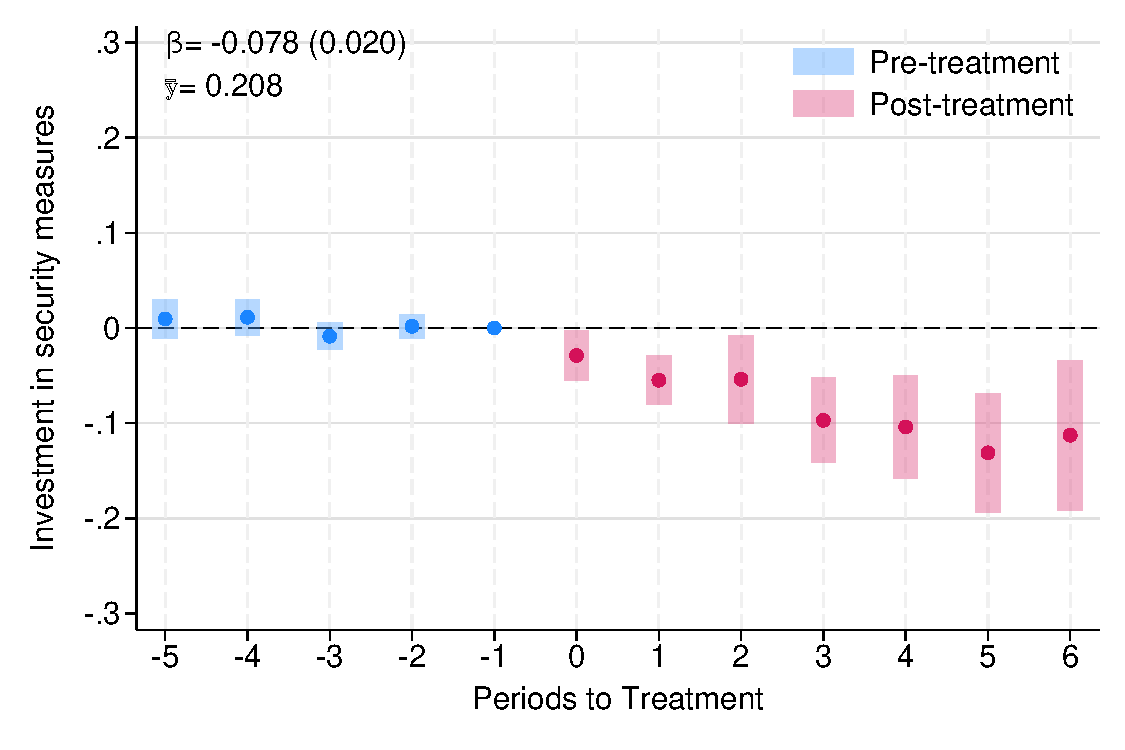
\includegraphics[width=\textwidth]{../manuscript/Graphs/DID2S_event_study_medidas_general_12.pdf}
        \caption{Gardner}
    \end{subfigure}
    \\[6pt]
    \begin{subfigure}{0.47\textwidth}
        \centering
        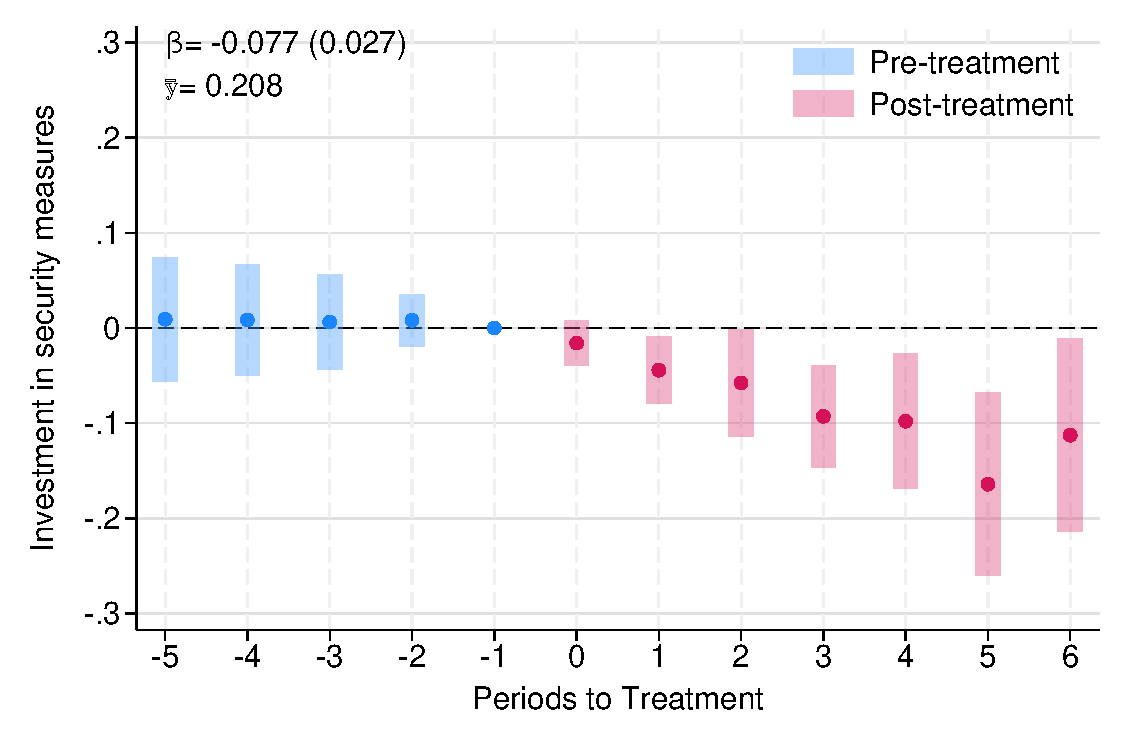
\includegraphics[width=\textwidth]{../manuscript/Graphs/JWDID_event_study_medidas_general_12.pdf}
        \caption{Wooldridge}
    \end{subfigure}
    \\[12pt]
    \begin{minipage}{0.99\textwidth}
    \footnotesize Notes: The figure reports event-study estimates of the effect of \emph{Plan Cuadrante} on the probability of adopting security measures in the last twelve months using the ENUSC survey, estimated with three alternative difference-in-differences estimators robust to staggered adoption: \citet{Chaisemartin} in panel (a), \citet{Gardner} in panel (b), and \citet{wooldridge2023simple} in panel (c). Each panel plots the estimated coefficient at each event time relative to treatment along with 95\% confidence intervals. Standard errors are clustered at the municipality level. The headline coefficient $\beta$ corresponds to the average post-treatment effect, and $\bar{y}$ denotes the never-treated mean of the outcome over the sample period.
    \end{minipage}
\end{figure}


% =============================================================================
% Administrative data (SPD municipality-level)
% =============================================================================


% ----- Reported crime --------------------------------------------------------
\begin{figure}[h!]
    \centering
    \caption[Effects of \emph{Plan Cuadrante} on Reported Crime Using Alternative Estimators]{Effects of \emph{Plan Cuadrante} on Reported Crime Using Alternative Estimators}
    \label{fig:alterestim_crime}
    \begin{subfigure}{0.47\textwidth}
        \centering
        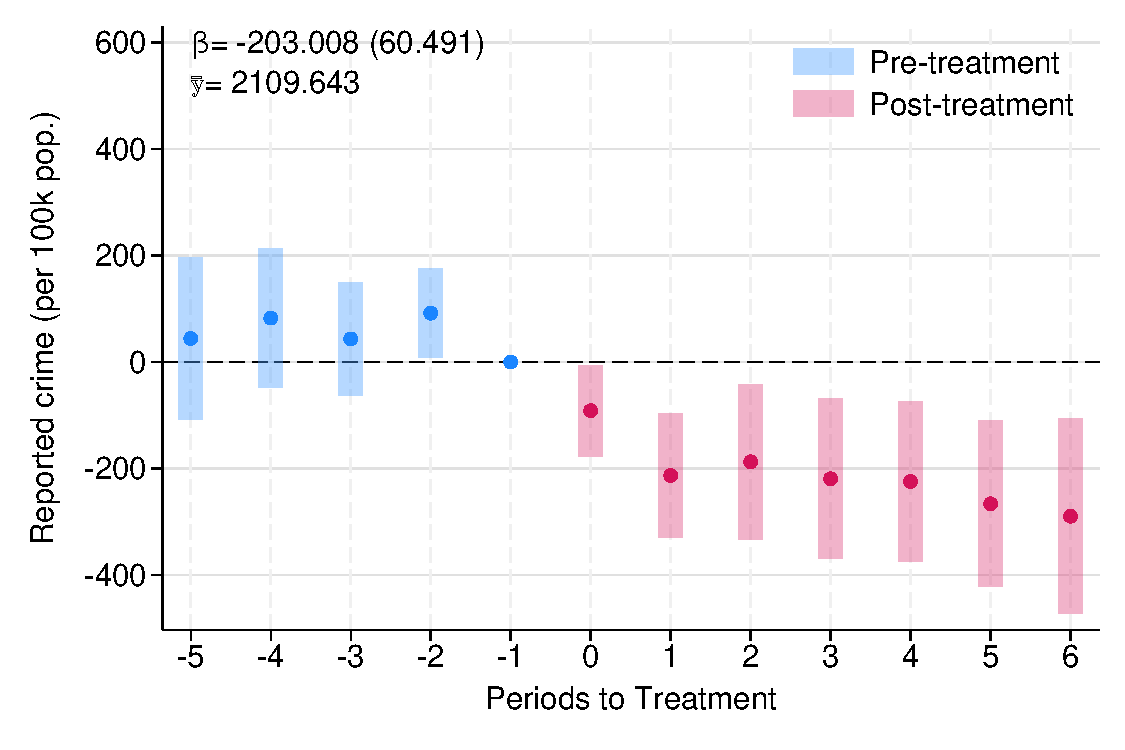
\includegraphics[width=\textwidth]{../manuscript/Graphs/CHDH_event_study_crime.pdf}
        \caption{Chaisemartin \& D'Hautfeuille}
    \end{subfigure}%
    \begin{subfigure}{0.47\textwidth}
        \centering
        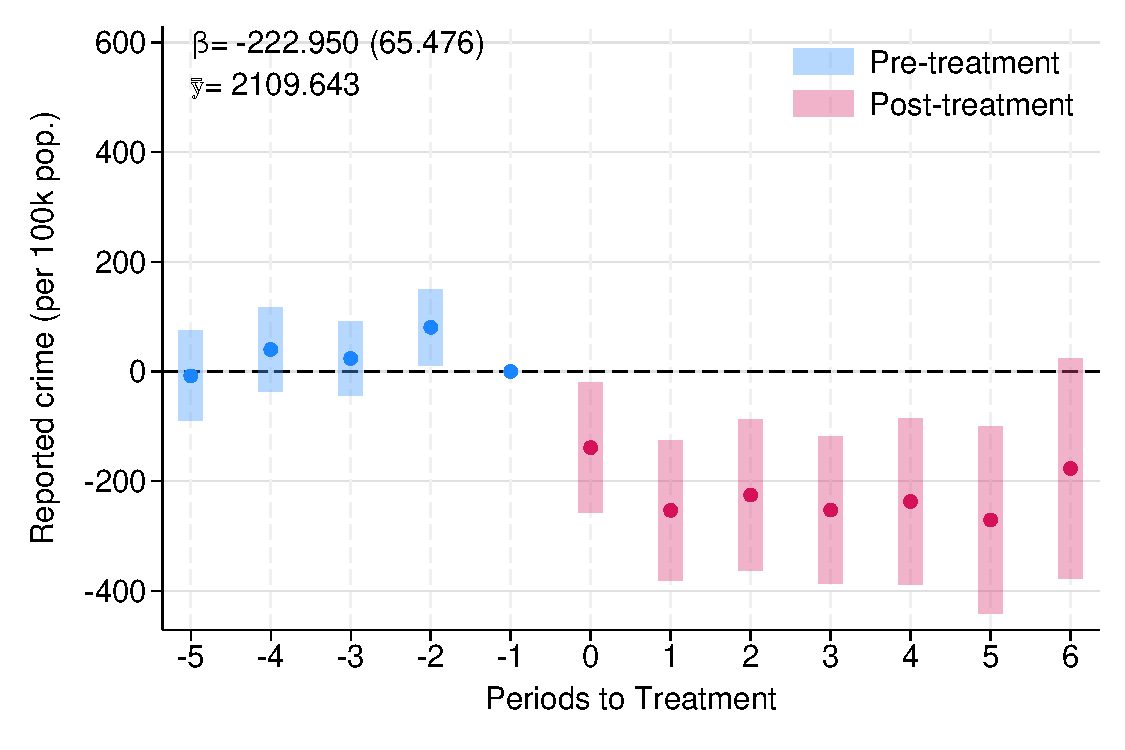
\includegraphics[width=\textwidth]{../manuscript/Graphs/DID2S_event_study_crime.pdf}
        \caption{Gardner}
    \end{subfigure}
    \\[6pt]
    \begin{subfigure}{0.47\textwidth}
        \centering
        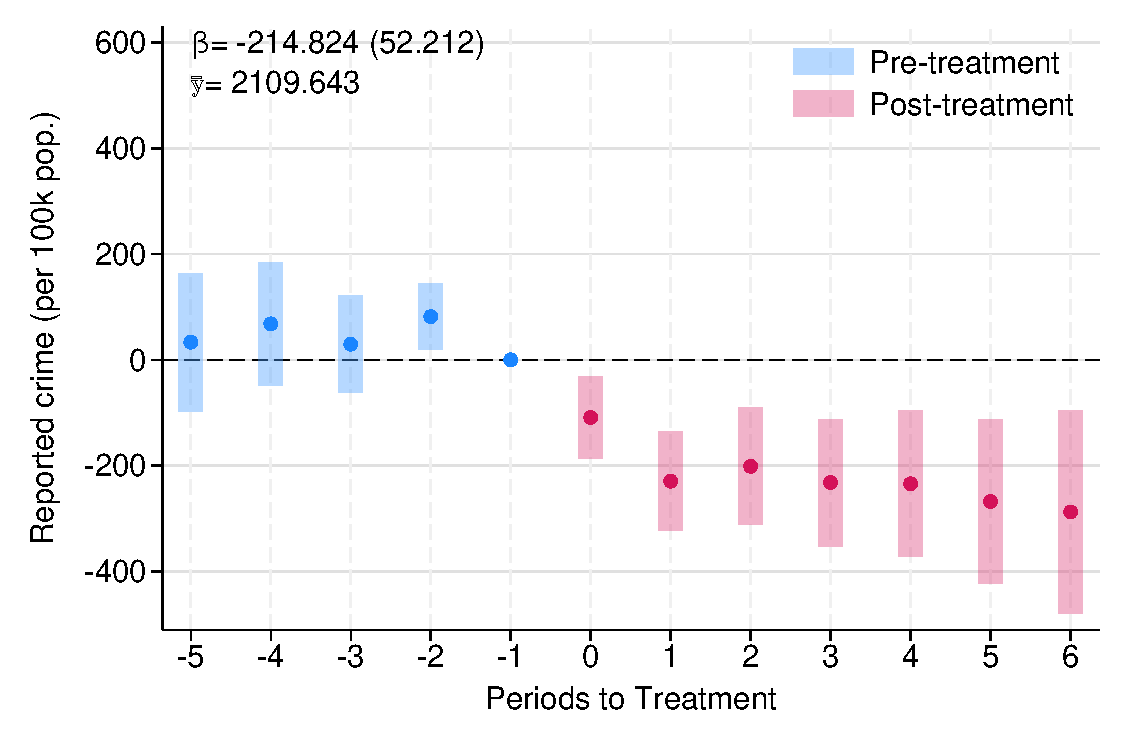
\includegraphics[width=\textwidth]{../manuscript/Graphs/JWDID_event_study_crime.pdf}
        \caption{Wooldridge}
    \end{subfigure}
    \\[12pt]
    \begin{minipage}{0.99\textwidth}
    \footnotesize Notes: The figure reports event-study estimates of the effect of \emph{Plan Cuadrante} on the number of crimes reported to the police in the municipality per 100,000 inhabitants using administrative data, estimated with three alternative difference-in-differences estimators robust to staggered adoption: \citet{Chaisemartin} in panel (a), \citet{Gardner} in panel (b), and \citet{wooldridge2023simple} in panel (c). Each panel plots the estimated coefficient at each event time relative to treatment along with 95\% confidence intervals. Standard errors are clustered at the municipality level. The headline coefficient $\beta$ is the equal-weighted average of the post-treatment effects from $t=0$ to $t=6$, and $\bar{y}$ denotes the never-treated mean of the outcome over the sample period.
    \end{minipage}
\end{figure}
